\section{Verification of LDA}
\begin{frame}
\frametitle{Correlation energy per electron}
\begin{figure}
    \centering
    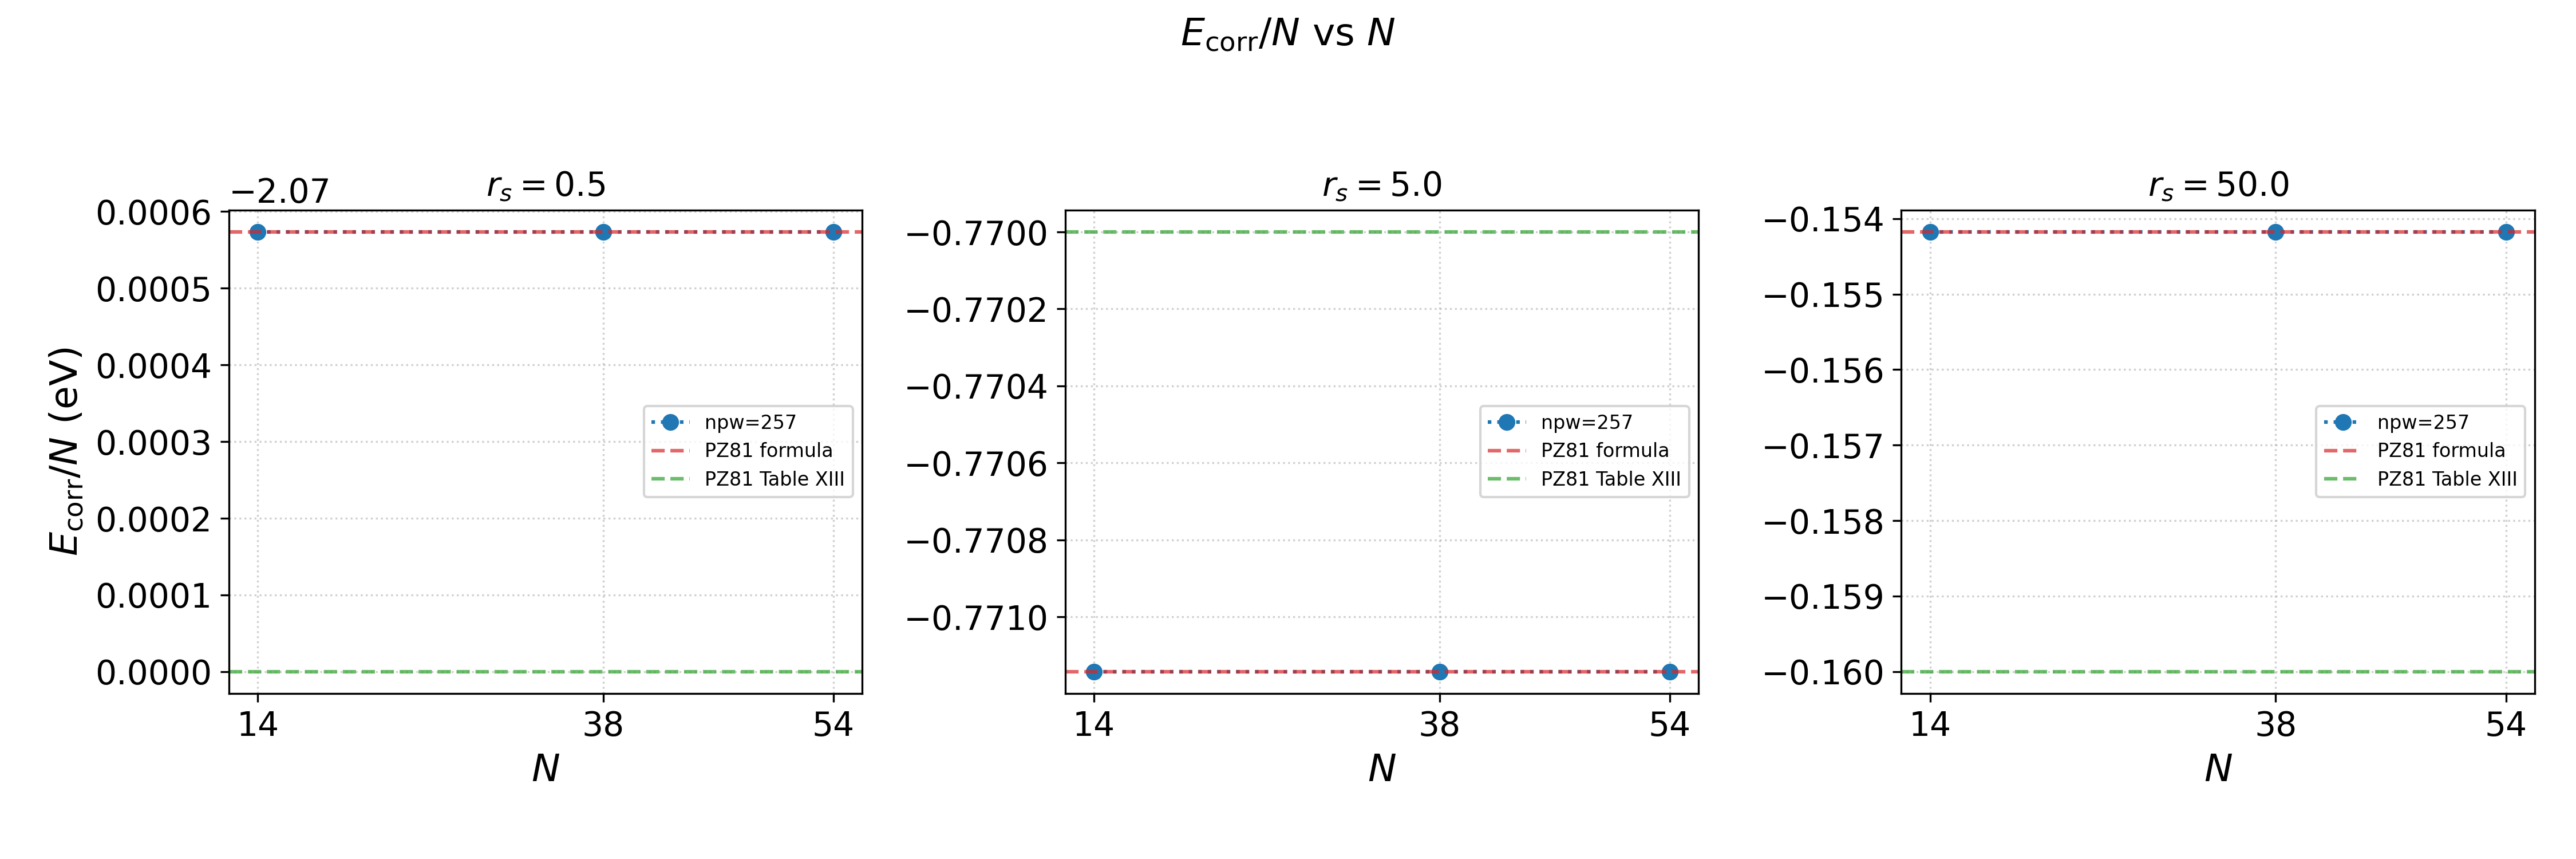
\includegraphics[width=\textwidth]{figs/lda_ecorr_perN_vs_N_multi_rs.png}
    \caption{To be compared with PZ81, Table XIII.}
    \label{fig:lda_ecorr_perN_vs_N_multi_rs}
\end{figure}
\end{frame}
\begin{frame}
\frametitle{Density as a function of $r_s$}
\begin{figure}
    \centering
    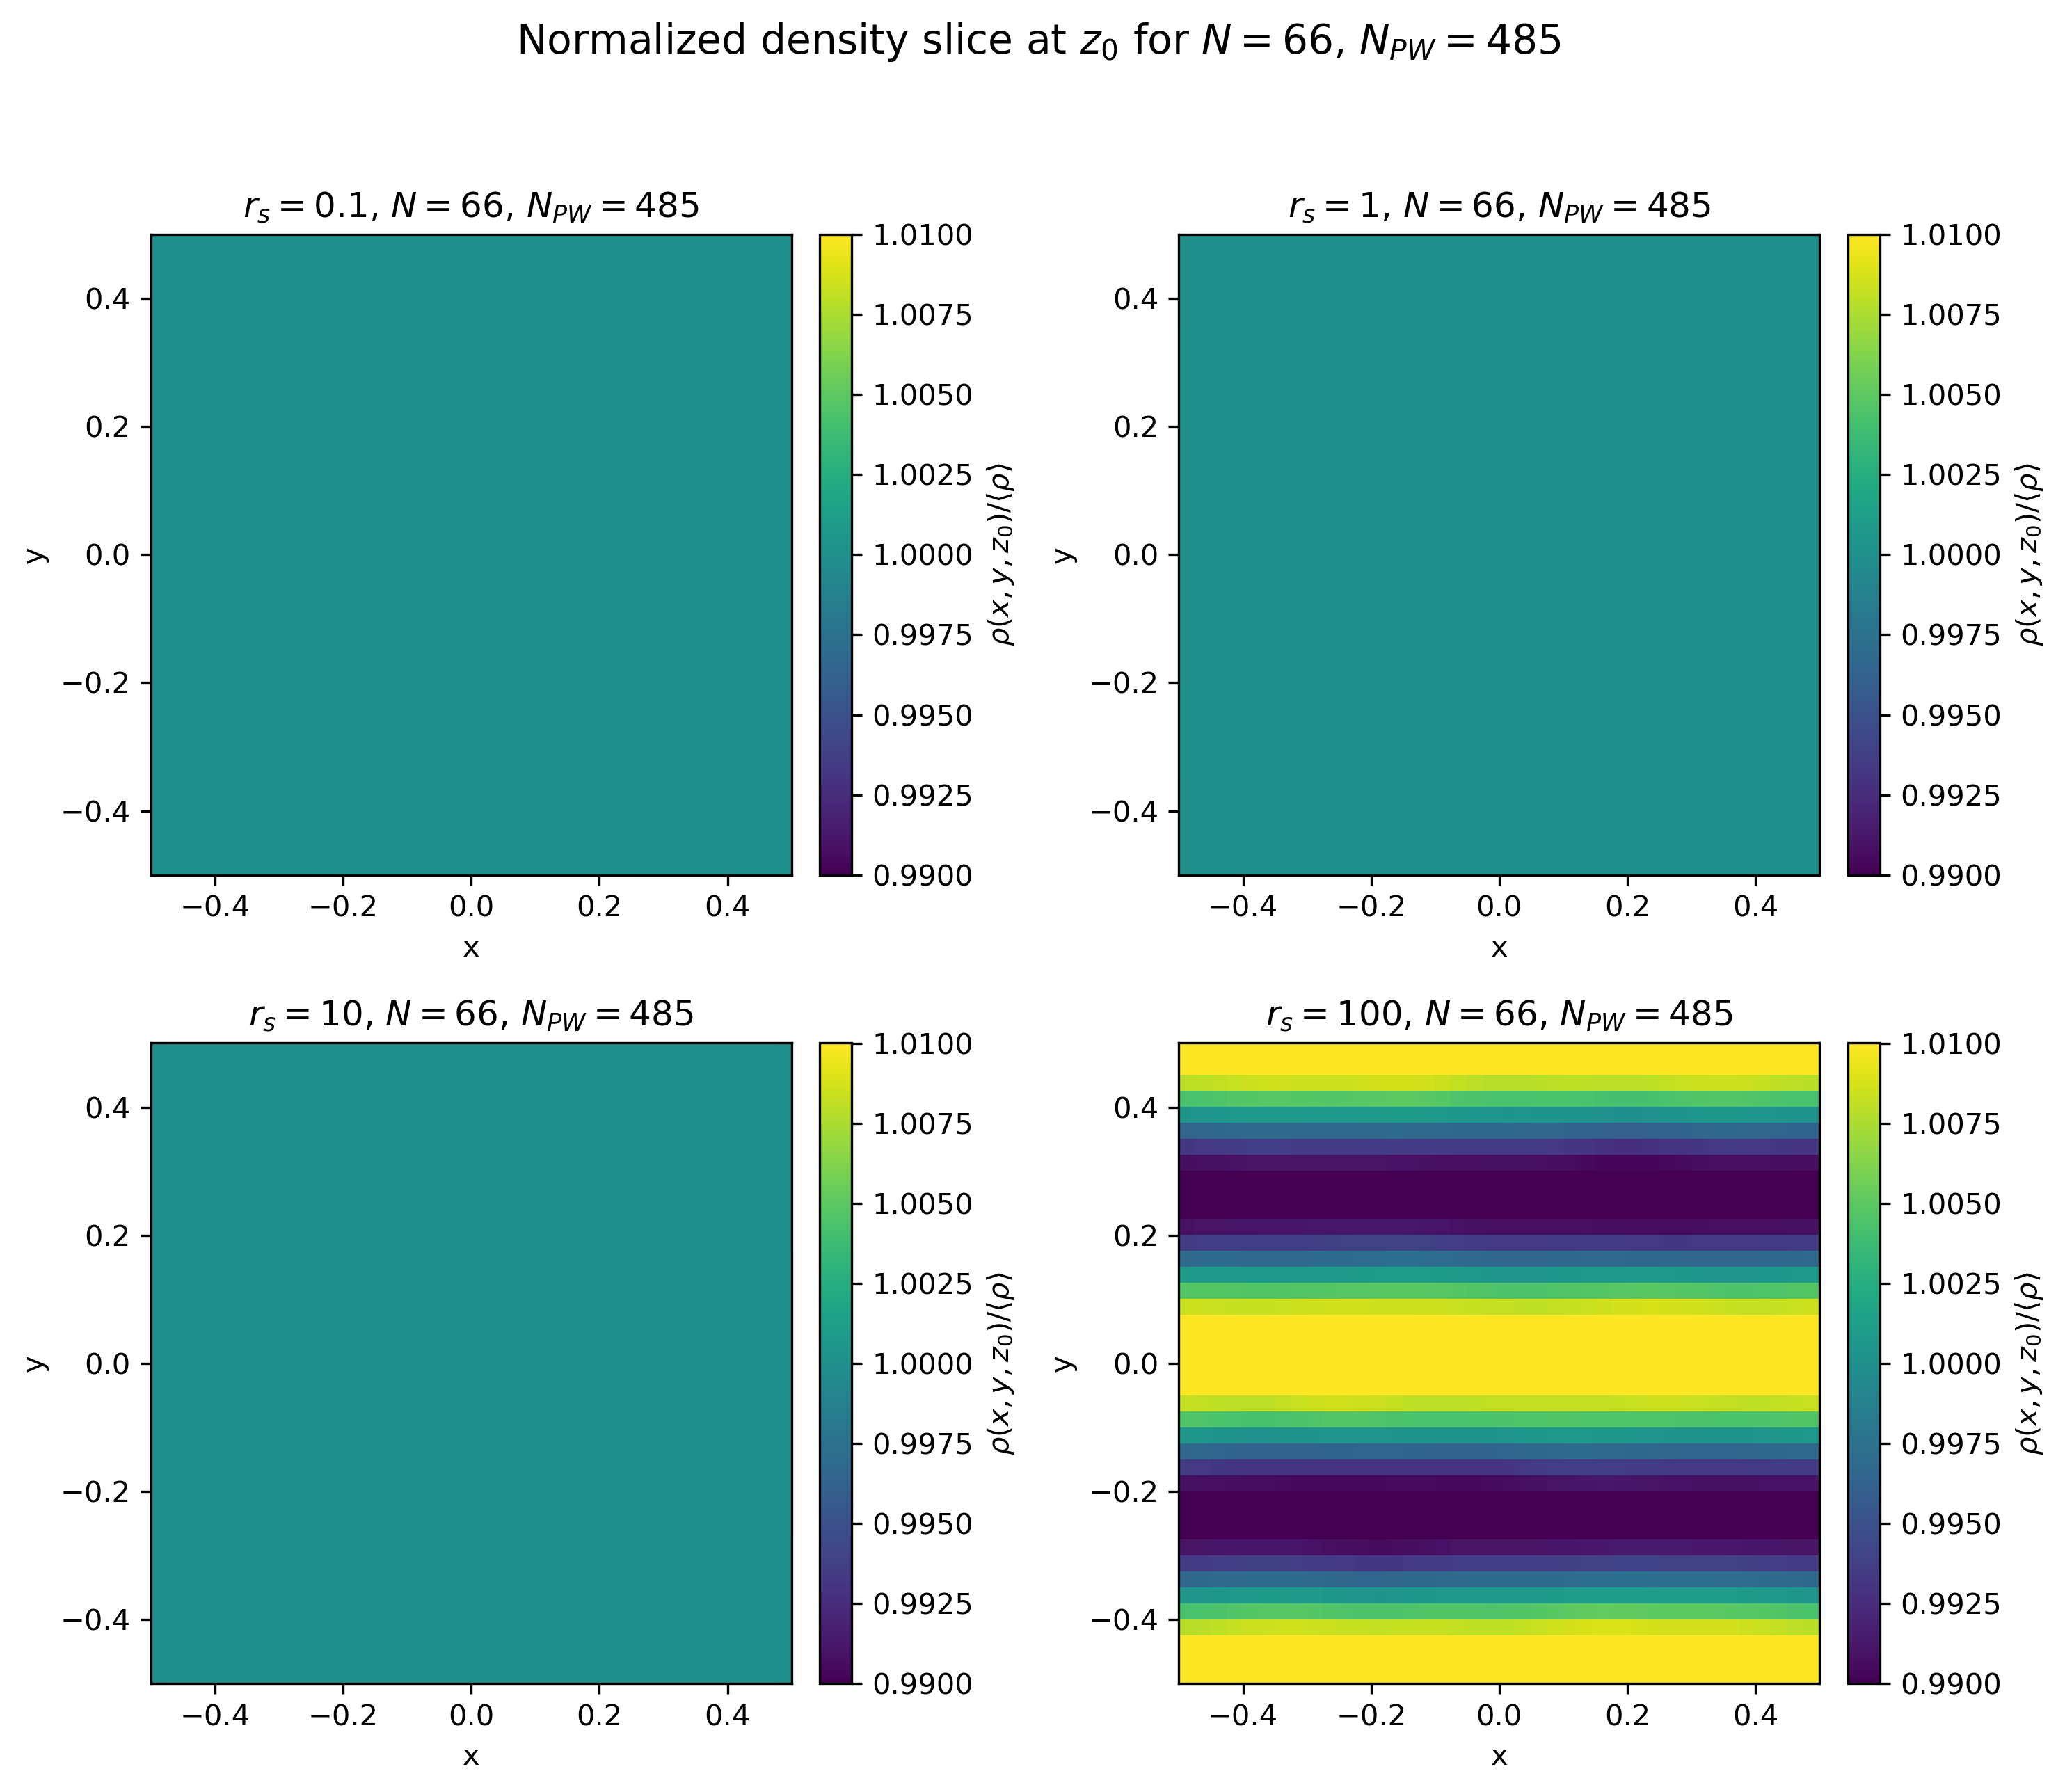
\includegraphics[width=0.75\textwidth]{figs/rho_slices_npw485_ne66.png}
\end{figure}
\end{frame}
\begin{frame}
\frametitle{Density as a function of $r_s$ continued}
\begin{figure}
    \centering
    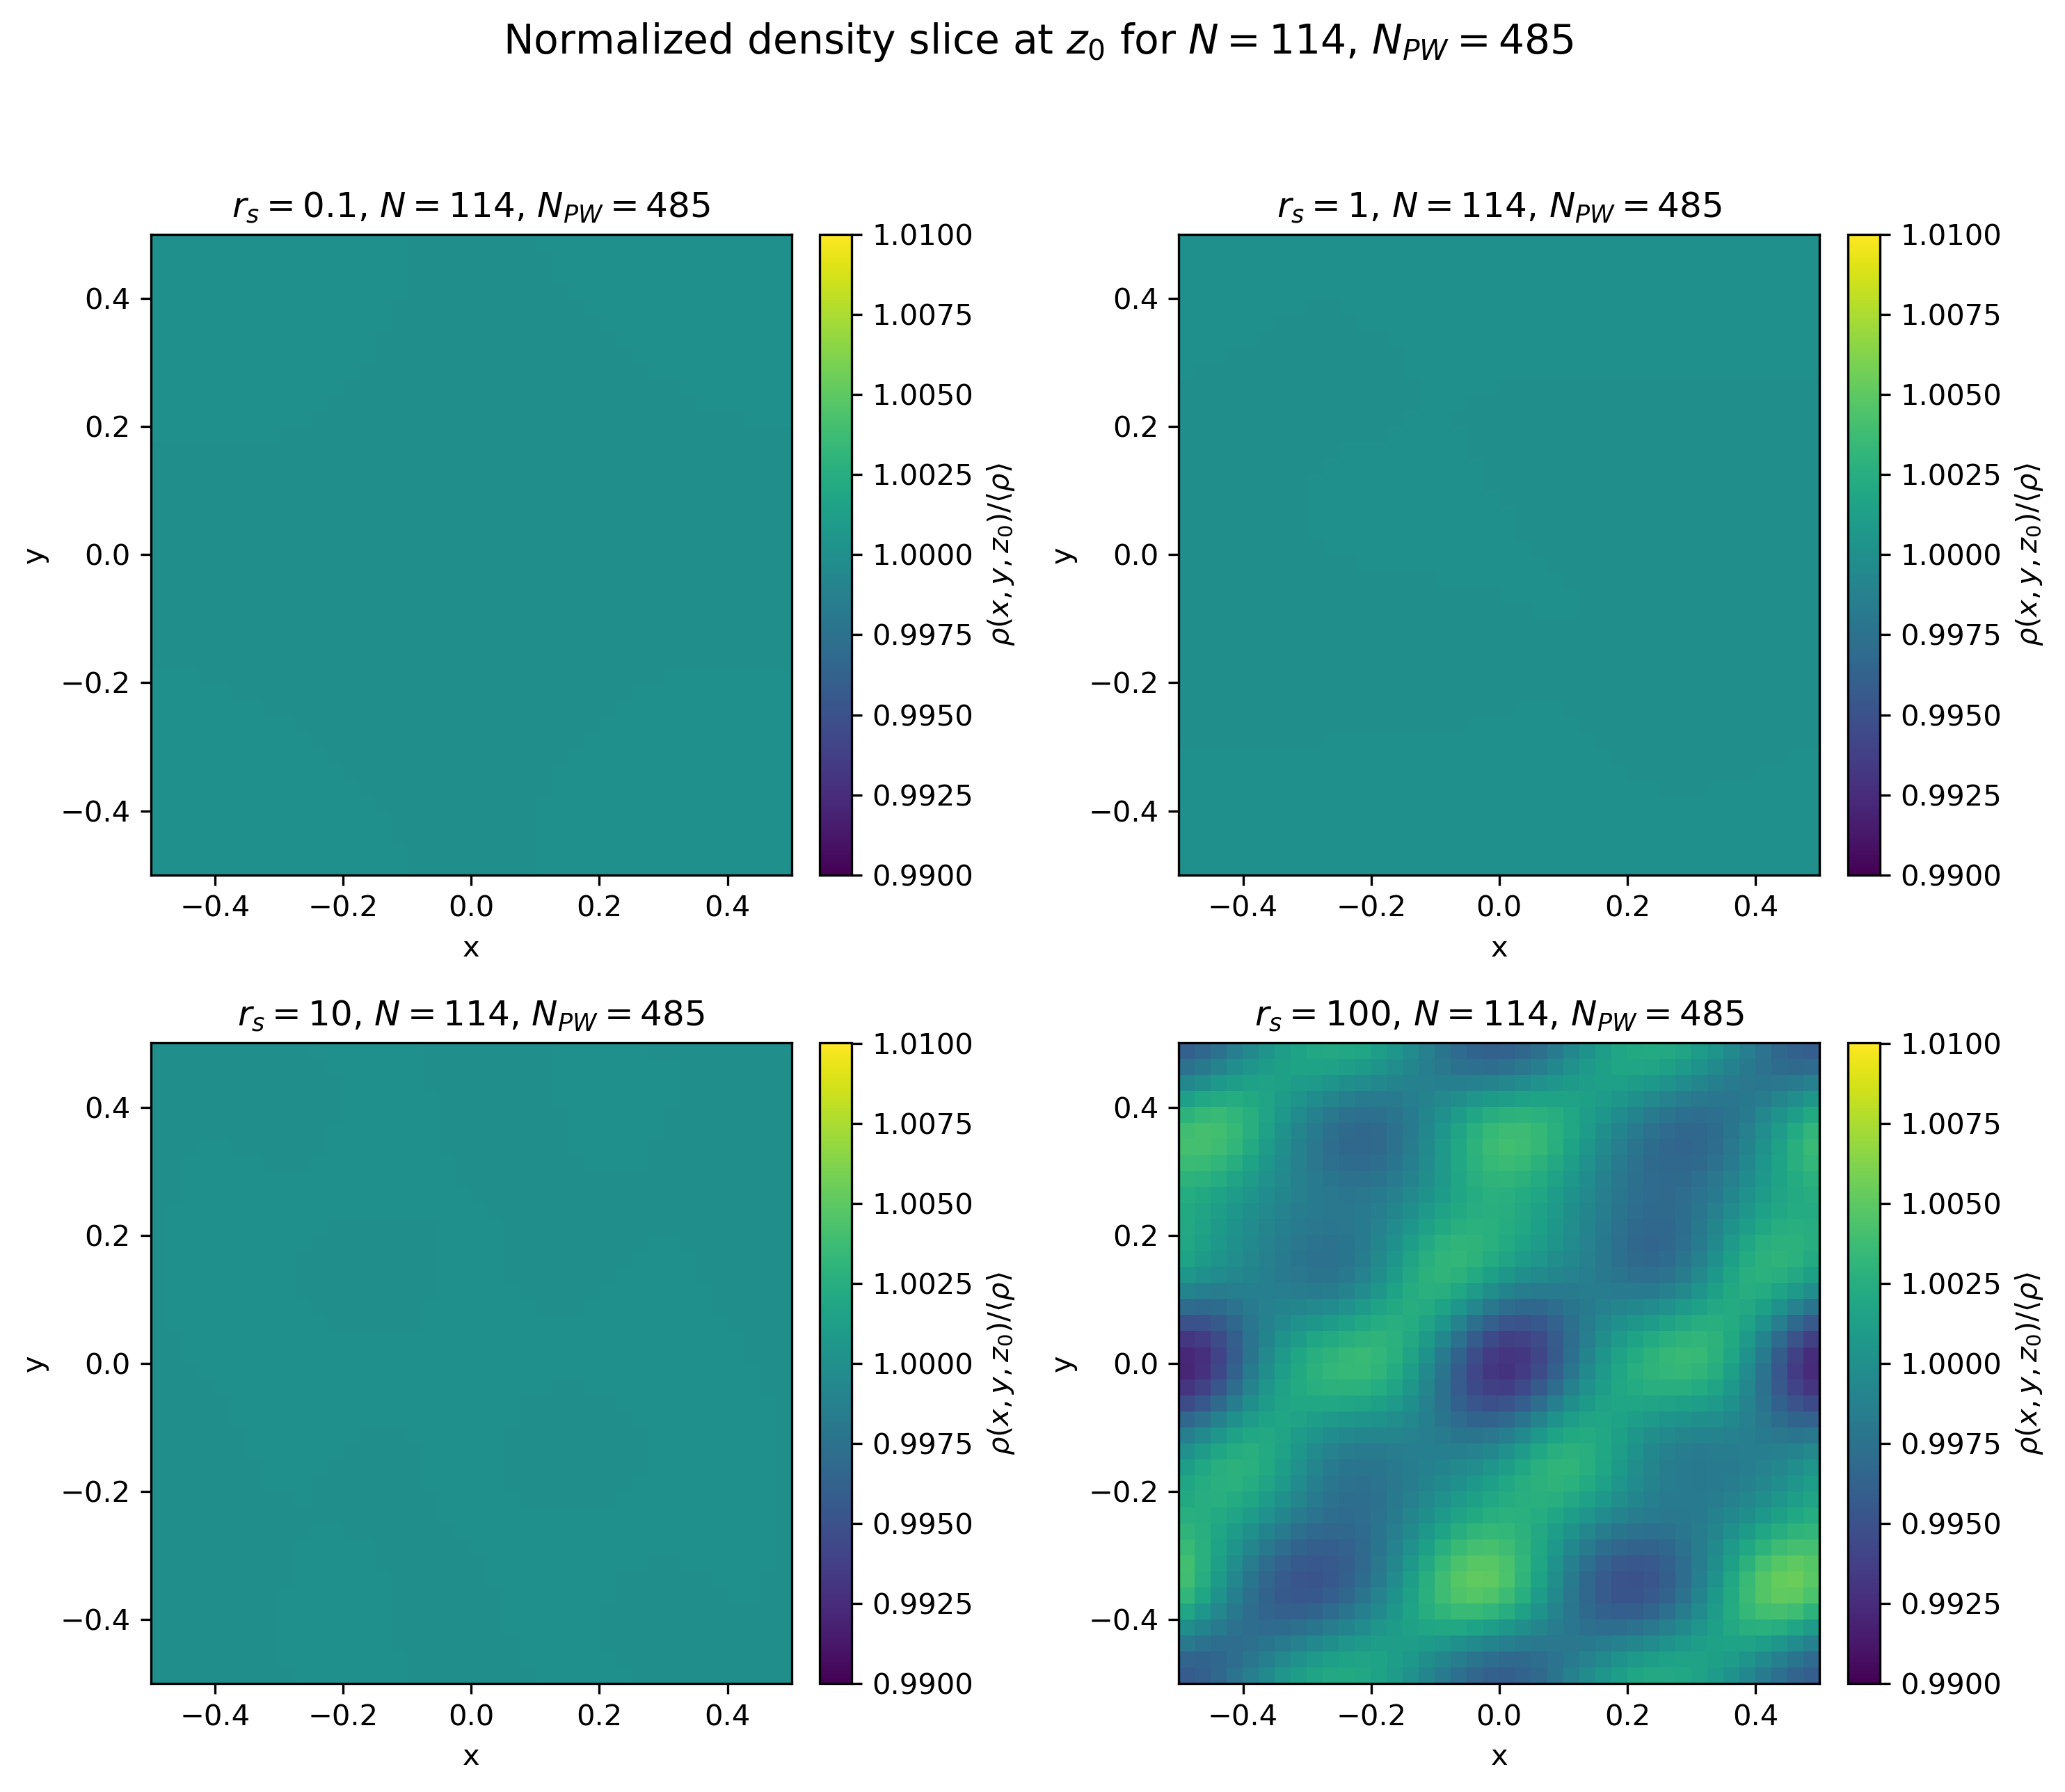
\includegraphics[width=0.75\textwidth]{figs/rho_slices_npw485_ne114.png}
\end{figure}
\end{frame}
\begin{frame}
\frametitle{Analysis of density slices}
Inhomogeneity at low density is observed, as expected.
\end{frame}
\section{Discussion of next steps}
\begin{frame}
\frametitle{Implementations of GW}
\begin{itemize}
    \item Implement GW with AC in Python; easiest to debug and check against PySCF that way.
    \item Nemo has been working on implementing GW with CD into C++. 
    \item Once I verify that my Python implementation of GW with AC is correct, the QCPBC infrastructure will already be there to add GW with AC also.
\end{itemize}
\end{frame}